\section{Evaluation}

The results of the PAN~2010 competition~\cite{Potthast2010b}
provide a benchmark of comparison for vandalism detection systems.
Although receiver operating characteristic was used to judge the
competition, the analysis by Potthast~\etal points to the conclusion
that the class imbalance between vandalized and regular edits
leads to better discriminatory power by precision-recall curves.
We evaluate our predictions using both methods and place them into
the context of other previously published results.

In Table~\ref{tab:vandalrep-confusion}, we present the confusion matrix
as determined by the Weka package.
There is a large class imbalance in the distribution of vandalism versus
regular edits, leading to a difficult prediction problem because of
needing to balance the predictive ability over the two classes.


For example, predicting that an edit is a regular contribution has a
precision of 95.4\% and recall of 98.4\%;
% Precision = tp / (tp + fp) = 29428 / (29428 + 1430) = 0.9537
% Recall = tp / (tp + fn) = 29428 / (29428 + 467) = 0.9844
in predicting vandalism, on the other hand, our model is only able
to achieve a precision of 67.2\% and recall of 40.1\%.
% Precision = tp / (tp + fp) = 957 / (957 + 467) = 0.6721
% Recall = tp / (tp + fn) = 957 / (957 + 1430) = 0.4009
Figure~\ref{fig:vandalrep-prcurve} shows the corresponding
precision-recall curve of the resulting predictions.
Using evaluation measures for classification problems, we get
the following performance for classifying edits as vandalism:
% Positive Predicive Value (Precision) = tp / (tp + fp)
% Sensitivity (Recall) = tp / (tp + fn)
% Specificity = tn / (tn + fp)
% Accuracy = (tp +tn) / (tp + tn + fp + fn)
\begin{align*}
\text{Positiv Predictive Value} &= 67.2\% \\
\text{Sensitivity} &= 40.1\% \\
\text{Specificity} &= 98.4\% \\
\text{Accuracy}    &= 94.1\% \\
\end{align*}

\begin{table}[b!tph]
  \begin{center}
    \begin{tabular}{| r | c c |}
      \hline
          & \multicolumn{2}{c|}{\textit{classified as}} \\
      \textit{actual class} & Regular & Vandalism \\
          \cline{2-3}
      Regular & 29428 & 467 \\
      Vandalism & 1430 & 957 \\
      \hline
    \end{tabular}
  \end{center}
  \caption[Confusion matrix for vandalism prediction]{%
    The confusion matrix for predicting edits of the PAN-WVC-10
    corpus as being regular edits or the work of vandals.
    Note that there is a large class imbalance in the distribution
    of how edits are truly classified.}
  \label{tab:vandalrep-confusion}
\end{table}

\begin{figure}[tbhp]
  \centering
  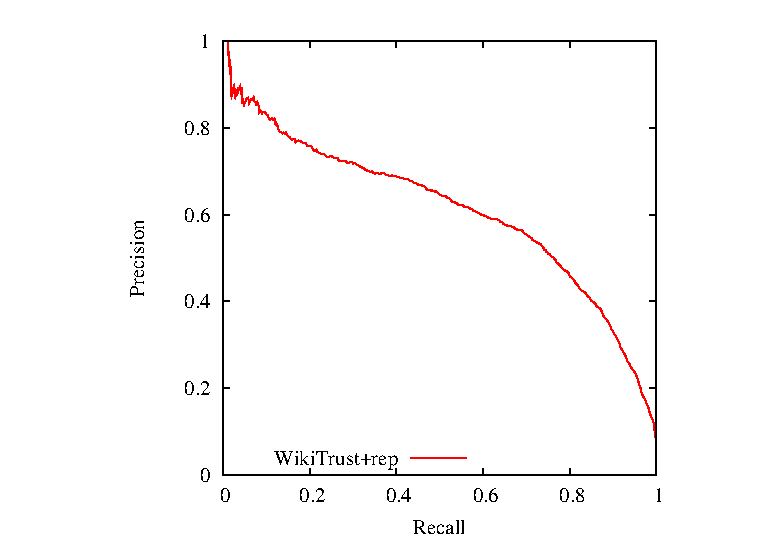
\includegraphics{part-Q10-vandalism/graph-wikitrust-pr}
  \caption[Precision-Recall curve for vandalism detection]{%
    Precision-Recall curve for a vandalism detection system based
    on features from the WikiTrust system, including reputation.
    This extends the previous WikiTrust results for immediate vandalism
    detection~\cite{Adler2010b} by including the reputation of authors
    at the time of each edit.}
  \label{fig:vandalrep-prcurve}
\end{figure}

\begin{table}[tbhp]
  \begin{center}
    \begin{tabular}{|l|c|c|}
      \hline
      \textbf{System} & \textbf{AUC-PR} & \textbf{AUC-ROC} \\
      \hline
      \hline
      PAN~2010 WikiTrust~\cite{Potthast2010b} & 0.49263 & 0.90351 \\
      STiki (Metadata)~\cite{Adler2011a} & 0.52534 & 0.91520 \\
      PAN 2010 WikiTrust + metadata~\cite{Adler2011a} & 0.61047 & 0.93647 \\
      PAN 2010 WikiTrust + reputation & 0.61152 & 0.94257 \\
      Mola-Velasco (NLP)~\cite{Adler2011a} & 0.73121 & 0.94567 \\
      Mola-Velasco + topic~\cite{Mola2011} & 0.7541 & \textit{n/a} \\
      PAN'10 Meta Detector~\cite{Potthast2010b} & 0.77609 & 0.95689 \\
      M-V + WT + STiki~\cite{Adler2011a} & 0.81829 & 0.96902 \\
      \hline
    \end{tabular}
  \end{center}
  \caption[Comparison of vandalism detection systems]{%
    Comparison of various vandalism detection systems.
    The results of this chapter are labeled ``PAN~2010 WikiTrust +
    reputation,'' to indicate that it builds on the results collected
    for and presented in~\cite{Potthast2010b} by including the
    author reputation score at the time of each edit.}
  \label{tab:vandalrep-context}
\end{table}

Understanding how to interpret these evaluative numbers is difficult,
so we provide the area under the precision-recall and receiver operating
characteristic curves in Table~\ref{tab:vandalrep-context}; this table
also contains those values for previously published results to give a
context for comparison.
From this data, we can answer our motivating question: does including
reputation as a feature result in better predictions?
Adding revision metadata features, and using the random forest
algorithm as a classifier, results in a significant improvement over the
original WikiTrust results~\cite{Adler2010b}.
Replacing the revision metadata features with author reputation does even better still,
answering our motivating question in the affirmative.

% 11027 anonymous edits
% 21255 non-anonymous edits
% =32283 total edits
% 1843 mispredictions, but probably only in test set


